\documentclass{beamer}
\usepackage{lmodern} % Add the lmodern package to fix missing font shapes
\usepackage{beamerthemeDHBW} % Include the package
\usepackage[overlay, absolute]{textpos}
\usepackage{bookmark}
\usepackage{pgfplots}
\usepackage{tikz}
\usepackage{amssymb} % Add the amssymb package to fix missing font shape
\usepackage{listings}
\newcommand{\internetadresse}{https://www.dhbw-stuttgart.de}
\pgfplotsset{compat=1.18}

\lstset{
    basicstyle=\ttfamily\scriptsize,
    keywordstyle=\color{blue},
    commentstyle=\color{green!60!black},
    numbers=left,
    numberstyle=\tiny\color{gray},
    frame=single,
    backgroundcolor=\color{lightgray},
    showspaces=false,
    showstringspaces=false,
    showtabs=false,
    breaklines=true,
    tabsize=4,
}


%Information to be included in the title page:
\title{Java-TX Compiler in Java-TX}
\author{Julian Schmidt}
\institute{DHBW Stuttgart}
\date{2024}

\usetheme{DHBW}

\begin{document}

\maketitle

\begin{frame}
    \frametitle{Agenda}
    \begin{enumerate}
        \item Motivation
        \item Aufbau der Umgebung
        \item Probleme
              \begin{enumerate}
                  \item Überschreibung von Methoden
                  \item Lambda Ausdrücke
              \end{enumerate}
        \item Bugs
    \end{enumerate}
\end{frame}

\begin{frame}
    \frametitle{Motivation}

    \begin{itemize}
        \item Welche Features fehlen noch in Java-TX?
        \item Welche Bugs gibt es?
        \item Wie performant is Java-TX für größere Projekte?
        \item Vorteile/Nachteile zu Java in der Praxis
    \end{itemize}

\end{frame}

\begin{frame}
    \frametitle{Motivation}
    \begin{center}
        \begin{tikzpicture}[scale=3]
            \draw (1,0) -- (0,0) -- (0,1) -- (3,1) -- (3,0) -- (2,0) -- (2, -1.1) -- (1, -1.1) -- cycle;
            \node at (0.5, 0.5) {JTX};
            \node at (1.5, -0.55) {JTX};
            \node at (2.5, 0.5) {BC};
            \draw (3.1,-1.1) -- (2.1,-1.1) -- (2.1,-0.1) -- (5.1,-0.1) -- (5.1,-1.1) -- (4.1,-1.1) -- (4.1, -2.2) -- (3.1, -2.2) -- cycle;
            \node at (2.6, -0.6) {JTX};
            \node at (3.6, -1.6) {JAVA};
            \node at (4.6, -0.6) {BC};
        \end{tikzpicture}
    \end{center}
\end{frame}

\begin{frame}[fragile]
    \frametitle{Aufbau der Umgebung}
    Erster Versuch mit make:
    \begin{lstlisting}
    # Use find to locate all .java and .jav files recursively
    JAVASOURCES := $(shell find $(SRCDIR) -name '*.java')
    JAVSOURCES := $(shell find $(SRCDIR) -name '*.jav')

    # Convert .java/.jav files to .class files with the same directory structure
    JAVACLASSES := $(patsubst $(SRCDIR)/%.java,$(DESTDIR)/%.class,$(JAVASOURCES))
    JAVCLASSES := $(patsubst $(SRCDIR)/%.jav,$(DESTDIR)/%.class,$(JAVSOURCES))

    # Rule for compiling .jav files
    $(DESTDIR)/%.class: $(SRCDIR)/%.jav
    java -jar $(JTX) -d "$(dir $@)" -cp "$(SRCDIR):$(DESTDIR):target/dependencies/" $<
    # Rule for compiling .java files
    $(DESTDIR)/%.class: $(SRCDIR)/%.java
	$(JC) -nowarn -d $(DESTDIR) -cp "$(SRCDIR):$(DESTDIR):target/dependencies/*" $(JFLAGS) $<
\end{lstlisting}
\end{frame}


\begin{frame}[fragile]
    Probleme:
    \begin{enumerate}
        \item javac compiliert und trackt Änderungen der Abhängigkeiten automatisch
        \item javac ist sehr langsam wenn für jede Datei einzeln aufgerufen
    \end{enumerate}
    \begin{columns}
        \begin{column}{0.5\textwidth}
            \begin{lstlisting}
javac src/main/java/de/dhbwstuttgart/typedeployment/TypeInsert.java
javac src/main/java/de/dhbwstuttgart/typedeployment/TypeInsertPlacer.java
...
javac src/main/java/Main.java
                \end{lstlisting}
            \sim{}5min
        \end{column}
        \begin{column}{0.5\textwidth}
            \begin{lstlisting}
javac src/main/java/de/dhbwstuttgart/typedeployment/TypeInsert.java src/main/java/de/dhbwstuttgart/typedeployment/TypeInsertPlacer.java ... src/main/java/Main.java
                \end{lstlisting}
            \sim{}2sec
        \end{column}
    \end{columns}
\end{frame}

\begin{frame}[fragile]{Bash Script}
    Gegeben: Quellverzeichnis, Zielverzeichnis
    \begin{enumerate}
        \item Suche rekursiv alle .java und .jav Dateien im Quellverzeichnis und speichere sie jeweils in einer Liste
        \item Überprüfe für jede Quelldatei, ob die zugehörige .class Datei im Zielverzeichnis existiert und ob die Zieldatei neuer als die Quelldatei ist
              \begin{itemize}
                  \item Wenn ja, gehe weiter zur nächsten Datei
                  \item Wenn nein, füge die Quelldatei zur Liste der zu kompilierenden Dateien hinzu
              \end{itemize}
        \item Rufe den Java-TX Compiler mit allen Dateien in der jav-Liste als Argumente auf
              \lstinline{java -jar $JAVATX_COMPILER_PATH -d $DESTDIR -cp "$SRCDIR:$DESTDIR:target/dependencies/" "${JAV_CHANGED[@]}"}
        \item Rufe den javac Compiler mit allen Dateien in der java-Liste als Argumente auf
              \lstinline{javac -d $DESTDIR -cp "$SRCDIR:$DESTDIR:target/dependencies/*" $JAVAC_FLAGS "${JAVA_CHANGED[@]}"}
    \end{enumerate}

\end{frame}

\begin{frame}[fragile]{Bugs}
    \begin{center}
        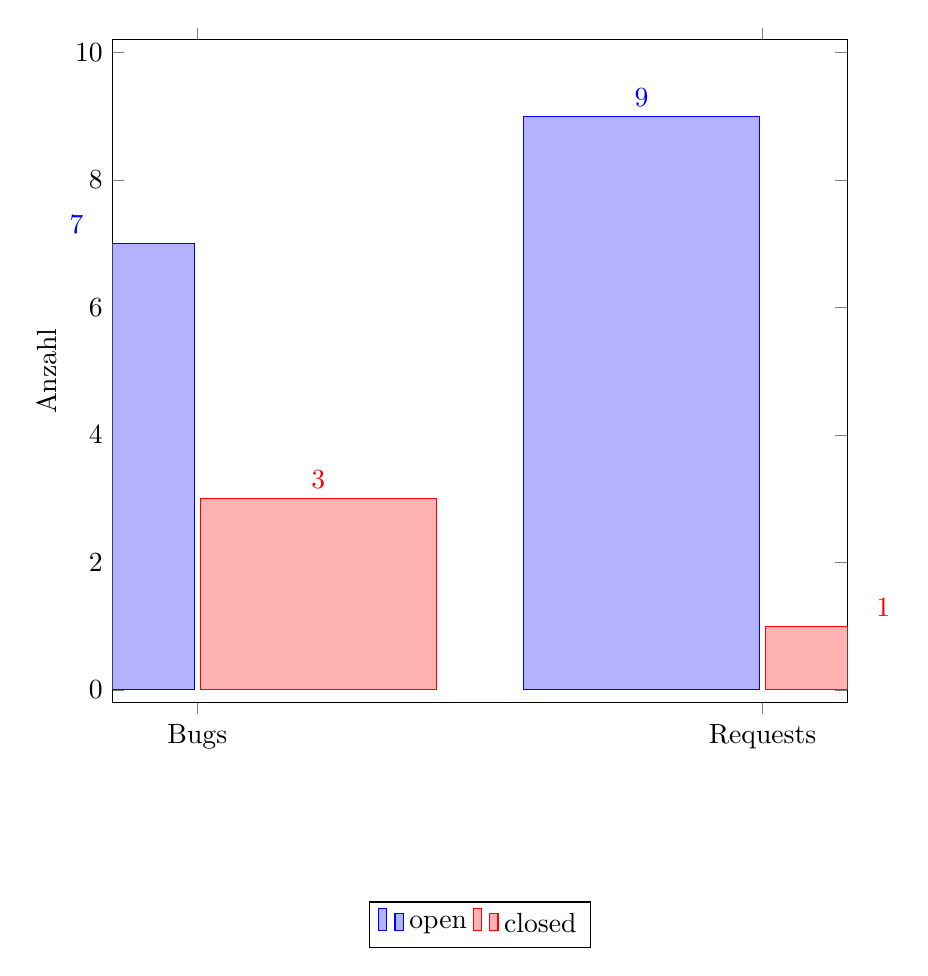
\begin{tikzpicture} \begin{axis}[ ybar, enlargelimits=0.15, legend style={at={(0.
                                5,-0.3)}, anchor=north,legend columns=-1}, ylabel={Anzahl}, symbolic x
                coords={Bugs,Requests}, xtick=data, nodes near coords, nodes near coords
                align={vertical}, width=0.9\textwidth, height=10cm, bar width=3cm] 
                \addplot coordinates {(Bugs,7) (Requests,9) };
                \addplot coordinates {(Bugs,3) (Requests,1) };
                \legend{open,closed}
            \end{axis} 
        \end{tikzpicture}
    \end{center}
\end{frame}

\end{document}
